% Abbildung 2.2 -- Energielandschaft V(phi) = -mgl*cos(phi), zur Illustration der
% instabilen Ruhelage (siehe AP5_Stichpunkte.md, Kapitel 2.1; Bereich [0,pi] passend zum
% Fliesstext in chapters/02_grundlagen.tex, der V(phi) nur auf [0,pi] einfuehrt).
%
% Eigenstaendig kompilierbar (standalone-Klasse) zur Pruefung -- einfach mit
% pdflatex/Overleaf direkt uebersetzen, es entsteht eine zugeschnittene PDF.
%
% GEOMETRIE-CHECK gegen protokoll.md §2.2 / Pendel_Herleitung_Ausfuehrlich.md §5:
%   V(phi) = -mgl*cos(phi)
%   phi = 0   -> V = -mgl  (Minimum -> stabile haengende Ruhelage)
%   phi = pi  -> V = +mgl  (Maximum -> instabile aufrechte Lage, das Regelziel)
% y-Achse ist auf mgl normiert (Achsbeschriftung zeigt "-mgl"/"mgl" statt Zahlenwerten,
% da m, g, l projektspezifische Parameter und keine fixen Zahlen sind).
%
% Einbindung: entweder diese Datei zu PDF kompilieren und in report/images/ ablegen
% + per \includegraphics einbinden, ODER \usepackage{pgfplots} + \pgfplotsset{compat=1.18}
% in main.tex ergaenzen und den tikzpicture-Rumpf per \input in
% chapters/02_grundlagen.tex einbinden (gleiches Vorgehen wie bei Abbildung 2.1).

\documentclass[tikz,border=8pt]{standalone}
\usepackage[T1]{fontenc}
\usepackage{amsmath}
\usepackage{pgfplots}
\pgfplotsset{compat=1.18}

\begin{document}
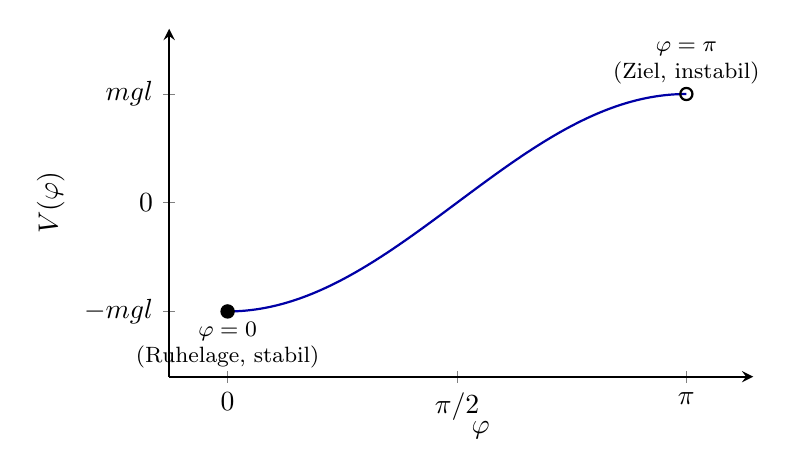
\begin{tikzpicture}
\begin{axis}[
    width=9cm, height=6cm,
    xmin=-0.4, xmax=3.6,
    ymin=-1.6, ymax=1.6,
    xtick={0,1.5708,3.1416},
    xticklabels={$0$,$\pi/2$,$\pi$},
    ytick={-1,0,1},
    yticklabels={$-mgl$,$0$,$mgl$},
    xlabel={$\varphi$},
    ylabel={$V(\varphi)$},
    axis x line=bottom,
    axis y line=left,
    xlabel style={anchor=west},
    ylabel style={anchor=south},
    clip=false,
    domain=0:3.1416,
    samples=150,
    thick,
]

% --- Energie-Landschaft ---
\addplot[blue!65!black, thick] {-cos(deg(x))};

% --- Stabiles Minimum (gefuellt), bei phi=0 ---
\addplot[only marks, mark=*, mark size=2.2pt, black] coordinates {(0,-1)};
% --- Instabiles Maximum (offen), bei phi=pi -- Ziel des Reglers ---
\addplot[only marks, mark=o, mark size=2.2pt, black, thick] coordinates {(3.1416,1)};

% --- Beschriftungen ---
\node[below, align=center, font=\footnotesize] at (axis cs:0,-1)
    {$\varphi=0$\\ (Ruhelage, stabil)};
\node[above, align=center, font=\footnotesize] at (axis cs:3.1416,1)
    {$\varphi=\pi$\\ (Ziel, instabil)};

\end{axis}
\end{tikzpicture}
\end{document}
